\section{Auswertung}
\label{sec:Auswertung}

%\begin{figure}[H]
%  \centering
%  \includegraphics[height=8cm]{Krause_Witthaus/Christopher_Lucas.Spe}
%  \caption{Die Drillachse.}
%  \label{fig:drill}
%\end{figure}


\subsection{Abschwächung des ersten Würfels}
Die gemessenen Zählraten $N$ des ersten Würfels und die daraus mit Gleichung (1)
bestimmten Abschwächungskoeffizienten sind in Tabelle 1 dargestellt.

\begin{table}[H]
  \centering
  \caption{Zählrate in Abhängigkeit der Projektion}
  \label{tab:Parameter}
  \begin{tabular}{c c c| c c }
    \toprule
    Projektion & $N$ & Fehler & $N_{Al}$ & Fehler  \\
    \midrule
        $I_1$    & 16161 & 152 & &   \\
        $I_2$    & 16165 & 151 & &   \\
        $I_3$    & 16218 & 151 & &   \\
        $I_4$    & 15596 & 151 & &   \\
        $I_5$    & 15662 & 151 & &   \\
        $I_6$    & 15899 & 152 & &   \\
        $I_7$    & 15997 & 153 & &   \\
        $I_8$    & 16187 & 152 & &   \\
        $I_9$    & 16213 & 153 & &   \\
        $I_{10}$ & 15509 & 151 & &  \\
        $I_{11}$ & 15725 & 151 & &   \\
        $I_{12}$ & 15605 & 152 & &   \\
    \bottomrule
  \end{tabular}
\end{table}



\begin{figure}
  \centering
  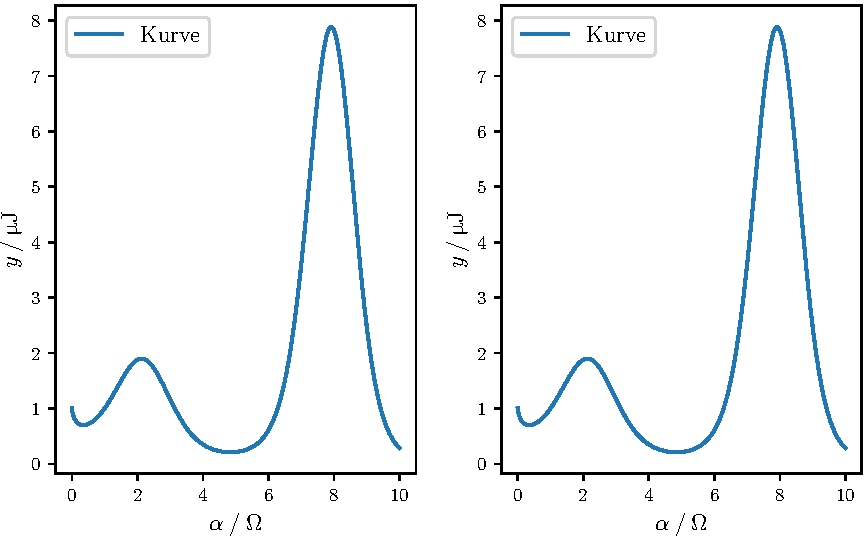
\includegraphics{plot.pdf}
  \caption{Plot.}
  \label{fig:plot}
\end{figure}
